\chapter{Non-Markovian Quantum State Diffusion}
\label{chap:nmqsd}
% * lin/nonlin Markovian SSE
% * little History
% * alternatives standard (projection?), pseudomodes
% * relevant/irre
%
% FIXME Citations
%
% TODO CHECK TENSES THOROUGHLY
% TODO CHECK THAT THERE IS \cc\zz EVERYWHERE
% TODO ALL IMAGES WITH SUBFIG-CAPTION!!!

The description of open quantum systems in terms of diffusive stochastic differential equations has a long tradition \cite{}.
At first, seen merely as a tool to unravel a given master equation of Lindblad type, it was realized later that they posses a strong microscopical foundation in terms of continuous measurements or memoryless quantum environments \cite{}.\\



% ✔ same applies to nmqsd unravelling: \cite{St96_lin_nmqsd}; microscopical theory: ...
%     => later is described in first section
% ✔ on its basis we derive a linear NMSSE, completely equivalent to micro. model, but numerical inferior
% * key point in hierachy later

Its non-Markovian generalization, the non-Markovian quantum state diffusion (NMQSD), took a quite similar path, which we roughly follow in this chapter:
Although first discovered as an unravelling for the Feynman-Vernon influence functional in terms of stochastic propagators \cite{St96_lin_nmqsd}, the corresponding non-Markovian stochastic Schrödinger equation (NMSSE) was derived based upon the standard open-system-model, which we \cm{recall} in \autoref{sec:nmqsd.model}.
Following the lines of Diósi, Strunz and Gisin \cite{DiSt97_nmsse,DiGiSt98_nmqsd,StDiGi99_nmq_traj} we derive both a linear and numerically superior non-linear version of the NMSSE in \autoref{sec:nmqsd.lin_nmsse} and~\ref{sec:nmqsd.nonlin_nmsse} respectively.

% * interpreation no so clear as markovian case
% * finite temperature, since derivation depends on vacuum initial bath state
%
% * study exemplary system, propose direct solution for T=0

\Autoref{sec:nmqsd.interpretation} is concerned with the question if our NMSSE has a physical interpretation or is just merely a computational tool.
%FIXME
\cm{Anschließend} we drop the requirement of zero initial temperature used in the \cm{vorherig} sections.
This chapter is \cm{abgeschlossen} by the treatment of an analytically soluble two-level system at zero temperature.\\

%FIXME Reference ok?
Most of the material covered can be found in reference \cite{St01_habil}, which we follow loosely.


%%%%%%%%%%%%%%%%%%%%%%%%%%%%%%%%%%%%%%%%%%%%%%%%%%%%%%%%%%%%%%%%%%%%%%%%%%%%%%%
\section{The Microscopical Model}
\label{sec:nmqsd.model}
% ✔ standard model (why oscillators, why linear coupling?)
% ✔ reservoir/environment
% ✔ initial states
%
% TODO Physical examples for such a model
% TODO Why harmonic oscillators for bosonic bath
% TODO Picture
%
%%%%%%%%%%%%%%%%%%%%%%%%%%%%%%%%%%%%%%%%%%%%%%%%%%%%%%%%%%%%%%%%%%%%%%%%%%%%%%%

It is the foremost goal of this work to obtain a dynamical equation for an open quantum system.
Nevertheless we introduce a full model of system and its environment first, the bosonic and non-relativistic standard model of an open quantum system extensively studied for example in the book of Weiss \cite{We99_dissipative_systems}.
There are three reasons for such a microscopical approach:
On one hand this serves the purpose to better understand the physical origin of macroscopical properties used to characterize the bath later on.
But more important, starting with a closed quantum system is the only strategy allowing us to derive the NMSSE from first principles, namely the Schrödinger equation.
%FIXME
A last argument in favor of the microscopic approach, PRODUCT STATES, ENTANGLEMENT, etc. ---we will not dwell on this any further.\\

As a starting point we consider an environment consisting of a finite number $N$ of uncoupled harmonic oscillators\footnote{%
  We use \quotes{environment}, \quotes{reservoir} and \quotes{bath} interchangeably, altough the later two suggest a large size compared to the system.
}.
A Generalization to an infinite number can be carried out formally along the same lines, replacing sums by infinite series or even integrals; a different approach within our framework is presented later.
The dynamics of both system and environment are then described by a unitary time evolution with the Hamiltonian
\begin{equation}
  \Htot = \Hsys \otimes \unit  +  \unit \otimes \Henv  +  \Hint,
  \label{eq:nmqsd.Htot}
\end{equation}
where $\Hsys$ and $\Henv$ are the free Hamiltonians of the system and the bath respectively.\footnote{%
  For some models like the damped harmonic oscillator \cite{CaLe83_diss_system} an additional renormalization term arises from the interaction.
  Nevertheless such a contribution is best attributed to $\Hsys$ since it only acts on the system's Hilbert space.
}
The latter is a sum over independent harmonic oscillators $\Henv = \sum_\lambda \omega_\lambda \adj{a}_\lambda a_\lambda$ expressed in bosonic ladder operators $a_\lambda$ and $\adj{a}_\lambda$ of the $\lambda$\th mode with frequency $\omega_\lambda$.
Treating a finite number of independent reservoirs poses no further difficulties and therefore is not elaborated in this section.

For the interaction between environment and system we confine ourselves to the case of linear coupling
\begin{equation}
  \Hint = \sum_\lambda \cc{g}_\lambda \, L \otimes \adj{a}_\lambda + g_\lambda \, \adj{L} \otimes a_\lambda.
  \label{eq:nmqsd.Hint}
\end{equation}
Here $L$ denotes the coupling operator in the system's Hilbert space and $g_\lambda \in \Complex$ the coupling strength of the $\lambda$\th mode.
% FIXME More details, taylor expansion?
Since in typical examples the coupling of an individual bath mode scales inversely with the environment size \cite{We99_dissipative_systems}, the linear coupling in~\ref{eq:nmqsd.Hint} seems reasonable for macroscopic large environments.
%FIXME stop repetition in "environment"
But our framework also incorporates small environments---even to the extreme of a single harmonic oscillator---with strong coupling as well.
For such cases the linearity needs to be imposed as another assumption of the model.

\begin{figure}
  \centering
  \documentclass{standalone}
\usepackage{amsmath}
\usepackage{tikz}
\usetikzlibrary{matrix}
\usetikzlibrary{calc}
\begin{document}
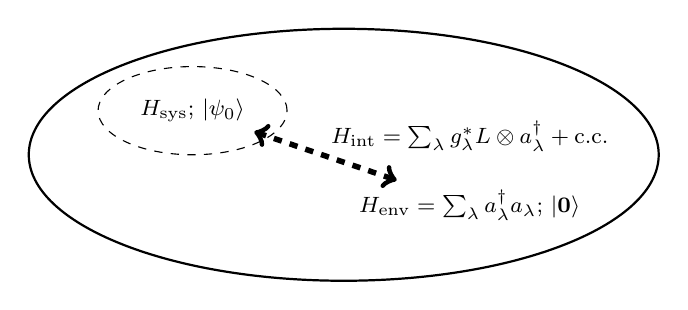
\begin{tikzpicture}[scale=.8]
  \node[align=center] at (-2.4, .7) (sys) {\footnotesize $H_\mathrm{sys}$; $|\psi_0\rangle$};
  \draw[dashed] (-2.4,.7) ellipse (1.5 and .7);
  \node[align=center,] at (2, -.8) (env) {\footnotesize $H_\mathrm{env}=\sum_\lambda a_\lambda^\dagger a_\lambda$;  $|\boldsymbol{0}\rangle$};

  \draw[thick] (0, 0) ellipse (5 and 2);

  \draw[<->, line width=2, dashed] (sys) -- (env);

  \node[align=right] at (2, .3) {\footnotesize $H_\mathrm{int} = \sum_\lambda g_\lambda^* L \otimes a_\lambda^\dagger + \mathrm{c.c.}$};

\end{tikzpicture}
\end{document}

  \caption{%
    Standard model of an open system immersed into a bosonic bath at zero temperature---this amounts to an initial product state $\ket{\psi_0}\otimes\ket{\vec 0}$.
    The environmental oscillators with frequencies $\omega_\lambda$ are described in terms of ladder operators $a_\lambda$ and $\adj{a}_\lambda$.
    A coupling operator $L$ mediates the influence of the environment.
  }
  \label{fig:nmqsd.open_system}
\end{figure}

Beside the Hamiltonian another important influence on the system's subdynamics is the initial state, specifically the initial entanglement between system and bath.
Throughout this work we only consider product initial conditions, where the bath is in the vacuum state with respect to all $a_\lambda$
\begin{equation}
  \ket{\Psi_0} = \ket{\psi_0} \bigotimes\limits_\lambda \ket{0_\lambda}.
  \label{eq:nmqsd.initial_conditions}
\end{equation}
Such a choice is not as restrictive as it seems on first glance: In \autoref{sec:nmqsd.temperature} we show how a thermal bath state can be mapped to~\ref{eq:nmqsd.initial_conditions}.
% FIXME cite Richard
However whether the NMSSE is applicable to initially entangled states is a question of current research.\\



To absorb the free dynamics of the environment in time dependent creation and annihilation operators, we switch to the interaction picture with respect to $\Henv$.
Since the bath operators only obtain an additional phase $\exp[\pm \ii \omega_\lambda t]$, the transformed Hamiltonian from \autoref{eq:nmqsd.Htot} reads\footnote{%
  We refrain from introducing another label to distinguish between time-evolution pictures---in what follows we always work in the interaction picture.
}
\begin{equation}
  \Htot(t) = \Hsys \otimes \unit  +  \sum_\lambda \left( \cc{g}_\lambda \exp[\ii \omega_\lambda t] \, L \otimes \adj{a}_\lambda + g_\lambda \exp[-\ii \omega t] \, \adj{L} \otimes a_\lambda \right).
  \label{eq:nmqsd.Htot}
\end{equation}
Our choice of unentangled initial conditions with a vacuum bath state ensures that the reduced density operator remains unaffected under the change of time-evolution picture.

It is instructive to rewrite the last equation using the operator valued force
\begin{equation}
  B(t)=\sum_\lambda g_\lambda a_\lambda \exp[-\ii\omega_\lambda t].
  \label{eq:nmqsd.force_operator}
\end{equation}
The total Hamiltonian then reads $\Htot(t) = \Hsys \otimes \unit  +  L \otimes \adj{B(t)}  +  \adj{L} \otimes B(t)$.
Already from this equation it can be seen, that the complete action of the environment on the system is encoded in the operators $B(t)$.
An important---and within our model the only---characteristic of them is the correlation function $\alpha(t-s) = \big\langle  (B(t) + \adj{B(t)})(B(s) + \adj{B(s)}) \big\rangle_\rho$ for an arbitrary bath state $\rho$.
For a thermal state at temperature $T$, the correlation function can be calculated analytically \cite{FeHi10_path_integrals}
\begin{equation}
  \alpha_T(t - s) = \sum_\lambda  \abs{g_\lambda}^2  \left( \operatorname{coth} \frac{\omega_\lambda}{2T} \, \cos \omega_\lambda (t-s)  -  \ii \sin \omega_\lambda(t-s) \right).
  \label{eq:nmqsd.thermal_correlation_function}
\end{equation}
Introducing the spectral density $J(\omega) = \sum_\lambda \abs{g_\lambda}^2 \delta(\omega - \omega_\lambda)$ and taking the limit $T \to 0$, the above equation can be rephrased as
\begin{equation}
  \alpha(t - s) = \qmean{B(t)\adj{B(s)}}_0 = \int_0^\infty J(\omega) \exp[-\ii\omega (t-s)] \dd \omega.
  \label{eq:nmqsd.correlation_function}
\end{equation}
In other words, the correlation function is simply given as one-sided Fourier transform of the spectral density.
% TODO Check this!
Of course this connection between response function and power spectrum---and its general form for $T\neq0$---is well known as fluctuation-dissipation relation.
Since a genuine physical spectral density is real, we require admissible correlation function to be hermitian $\alpha(-t) = \cc{\alpha(t)}$.\\

% TODO Types of correlation function, incommensurate frequencies, generalization --> contiuum-approximation, exp. decay, Markov, inclussion of negative frequencies,


%%%%%%%%%%%%%%%%%%%%%%%%%%%%%%%%%%%%%%%%%%%%%%%%%%%%%%%%%%%%%%%%%%%%%%%%%%%%%%%
\section{Linear NMSSE}
\label{sec:nmqsd.lin_nmsse}
% ✔ Bargman States, hilbert space valued functions
% ✔ derivation
% * problems, non-locality in noise
% ✔ reduced density operator
% * relative state --> interpretation; but also connection with H_s valued functions
% ✔ zero temperature, importance for calculations
% * quantum trajectory Carmichael
%
% TODO relation to unravelling
% TODO Make clear that interaction picture does not matter for purely system observables
%
%%%%%%%%%%%%%%%%%%%%%%%%%%%%%%%%%%%%%%%%%%%%%%%%%%%%%%%%%%%%%%%%%%%%%%%%%%%%%%%

The linear non-Markovian stochastic Schrödinger equation derived in this section is an equivalent reformulation of the interaction-picture Schrödinger equation
\begin{equation}
  \partial_t \ket{\Psi_t} = -\ii \Htot(t) \ket{\Psi_t}, \qquad \ket{\Psi_0} = \ket{\psi_0} \otimes \ket{0},
  \label{eq:nmqsd.schroedinger_ia}
\end{equation}
corresponding to the model of the last section:
Expressing the bath degrees of freedom in the Bargmann Hilbert space of anti-holomorphic functions\cite{Ba61_coherent_states} provides a representation that is well suited for a Monte-Carlo treatment.
To this end we introduce the unnormalized coherent state $\ket{z_\lambda} = \exp(z_\lambda \adj{a}_\lambda)\ket{0_\lambda}$ for each mode with resolution of the identity for the environment
\begin{equation}
  \unit = \int \frac{\exp[-\abs{\zz}^2]}{\pi^N} \, \ket{\zz}\bra{\zz} \dd^{2N}z,
  \label{eq:nmqsd.identity}
\end{equation}
Here we employ the shorthand notation $\ket{\zz} = \bigotimes_\lambda \ket{z_\lambda}$ and the \quotes{volume} integration measure for $N$ complex numbers $\dd^{2N}z = \prod_\lambda \dd\Re z_\lambda \dd\Im z_\lambda$.
Throughout this work the finite bath is often replaced by a continuum of oscillators; therefore we simply write $\mudz = \pi^{-N} \exp(-\abs{\vec z}^2) \dd^{2N}z$ to drop an explicit reference to $N$.
% TODO Rigorous existence?

\Autoref{eq:nmqsd.identity} allows us to express the full state in a time-independent environment basis
\begin{equation*}
  \ket{\Psi_t} = \int \ket{\psi_t(\cc\zz)} \otimes \ket{\zz} \mudz.
\end{equation*}
For the following derivation it is crucial to notice that the Bargmann transform $\zz \mapsto \psi_t(\cc\zz)$ is an anti-holomorphic function with values in the system's Hilbert space $\HHsys$.
Naturally it is equivalent to any other representation of the full state $\ket{\Psi_t}$.
As the coherent states are not orthogonal, but rather satisfy $\braket{\vec w}{\vec z} = \exp(\sum_\lambda \cc w_\lambda z_\lambda)$, the reduced density operator, obtained by tracing over the bath degrees of freedom, reads
%TODO Does this need a prove?
\begin{equation}
  \rho(t) = \Tr_\mathrm{env} \ket{\Psi_t}\bra{\Psi_t}
          = \int \ket{\psi_t(\cc\zz)}\bra{\psi_t(\cc\zz)} \mudz.
  \label{eq:nmqsd.reduced_matrix}
\end{equation}

% Only Schrödinger equation point of view!
% FIXME Citations of Strunz papers
After fixing the kinematic structure, the next step is to rewrite the dynamical equation:
The representation of the ladder operators follow from the usual rules $\bra\zz \adj{a}_\lambda = \cc z_\lambda \bra\zz$ and $\bra\zz a_\lambda = \partial_{\cc z_\lambda} \bra\zz$.
These expressions applied to \autoref{eq:nmqsd.schroedinger_ia} give us the system-bath Schrödinger equation in the transformed space
\begin{equation}
  \partial_t \psi_t(\cc\zz) = -\ii\Hsys\psi_t(\cc\zz)  -  \ii L \sum_\lambda \cc g_\lambda \exp[-\ii\omega_\lambda t] \cc z_\lambda \, \psi_t(\cc\zz)  -  \ii \adj{L} \sum_\lambda g_\lambda \exp[\ii\omega_\lambda t] \, \frac{\partial \psi_t}{\partial z_\lambda}(\cc\zz).
  \label{eq:nmqsd.hamiltonian_microsopic}
\end{equation}
Introducing an effective driving process like in \autoref{eq:nmqsd.force_operator}
\begin{equation}
  \ZZ_t(\cc\zz) = - \ii \sum_\lambda \cc g_\lambda \exp[\ii \omega_\lambda t] \cc z_\lambda
  \label{eq:nmqsd.stochastic_process}
\end{equation}
allows us to combine the effect of the first bath-interaction term into a single multiplication operator---or process for reasons explained in the next paragraph.
% FIXME Proof of functional chain rule?
A similar conversion works for the second term as well with the help of the functional chain rule $\frac{\partial}{\partial \cc z_\lambda} = \int \frac{\partial \ZZ_s}{\partial\cc z_\lambda} \frac{\delta}{\delta \ZZ_s} \dd s$.
Combined our new equation of motion ---the non-Markovian stochastic Schrödinger equation---reads
\begin{equation}
  \partial_t \psi_t = -\ii\Hsys\psi_t  +  L\ZZ_t\psi_t  -  \adj{L} \int_0^t \alpha(t-s) \frac{\delta \psi_t}{\delta \ZZ_s} \dd s.
  \label{eq:nmqsd.nmsse}
\end{equation}
As we shown in \autoref{sub:nmqsd.interpretation.unitary_view}, the integral boundaries arise due to the initial conditions~\ref{eq:nmqsd.initial_conditions}; a less formal argumentation goes as follows:
By construction of our processes~\ref{eq:nmqsd.stochastic_process} an initial state $\ket{\psi_0}\otimes\ket{0}$ translates to an initial $\psi_0(\ZZ)$ that is completely independent of any noise.
Then causality implies that $\psi_t$ can only depend on $\ZZ_s$ for $0 \le s \le t$.\\



Up to this point we have merely rewritten the original Schrödinger equation~\ref{eq:nmqsd.schroedinger_ia} to an equivalent form:
The original system-bath product Hilbert space $\HHsys \otimes \HHenv$ is replaced by a Hilbert space of $\HHsys$-valued functions.
A different attitude is quite fruitful, especially with a numerical solution of the NMSSE in mind:
\Autoref{eq:nmqsd.reduced_matrix} can be rewritten as $\rho_t = \E[\ket{\psi_t}\bra{\psi_t}]$, where $\E$ denotes the average over $\mudz = \pi^{-N} \exp(-\abs{\vec z}^2) \dd^{2N}z$.
Put differently the reduced density matrix $\rho_t$ arises by averaging over the stochastic pure state projectors $\ket{\psi_t(\cc\zz)}\bra{\psi_t(\cc\zz)}$ with Gaussian weight $\mudz$.
Hence we regard \autoref{eq:nmqsd.nmsse} as a stochastic differential equation for individual realisations $\psi_t(\cc\zz)$.
We refer to the later either as system state relative to $\ket{\zz}$ or, in the spirit of the stochastic Schrödinger equations emerging from continuous measurement theory \cite{Ca93_quantum_optics}, as quantum trajectory.

In this approach the driving force $\ZZ_t$ is implemented as classical stochastic process defined by the concrete version~\ref{eq:nmqsd.stochastic_process} and the underlying probability measure $\mu$.
It is a complex Gaussian process uniquely characterized by its expectation value and covariances
\begin{equation}
  %FIXME Z_t compared to \ZZ_s looks strange! The subscript is moved.
  \E\,Z_t = 0, \quad \E\,Z_t Z_s =0, \quad\mbox{and}\quad \E\,Z_t \ZZ_s = \alpha(t-s),
  \label{eq:nmqsd.process_properties}
\end{equation}
where $\alpha$ is the zero-temperature correlation function~\ref{eq:nmqsd.correlation_function} for $J(\omega) = \sum_\lambda \abs{g_\lambda}^2 \delta(\omega - \omega_\lambda)$.
By virtue of the initial conditions, $\psi_t$ depends on $\zz$ only through the driving process; thus we can drop the coherent state labels and simply write $\psi_t(\ZZ)$ denoting the trajectory corresponding to a realisation $\ZZ(\cc\zz)$.
It is this alternative point of view that makes the NMSSE-approach so powerful:
The entire influence of the environment is encoded in a complex function $\alpha$, which acts both as correlation function for the driving noise $\ZZ$ and as memory kernel for the damping term.
A generalization to an arbitrary number of bath-oscillators is now straightforward: simply replacing the correlation function allows an unified description of arbitrary harmonic environments.

Except in the limit $\alpha(t) \propto \delta(t)$, elaborated in the next paragraph, the driving process $\ZZ_t$ is correlated for different times.
This non-Markovian behavior, which makes a complete understanding of the dynamics highly desirable for application but also considerably harder, shows up in the equation of motion~\ref{eq:nmqsd.nmsse} as well.
The damping term contains the functional derivative over the whole timespan and therefore takes the complete history of $\psi_t(\ZZ)$ into account.
In its own right the derivative is just as problematic:
% FIXME Quite long sentence!
Since its computation requires not only the single realisation $\ZZ$, but in some sense all adjacent ones as well, it seems questionable to regard the NMSSE~\ref{eq:nmqsd.nmsse} as a genuine stochastic differential equation \cite{GaWi02_real_nmsse}.
% FIXME DOOMED???
Even from the purely pragmatic point of view both kinds of non-local behavior complicate a direct numerical simulation of the NMSSE, if not making it completely impracticable.
Nevertheless there are two quite distinct solutions as shown in \autoref{sub:nmqsd.lin_nmsse.convolutionless} and \autoref{chap:num}.


%%%%%%%%%%%%%%%%%%%%%%%%%%%%%%%%%%%%%%%%%%%%%%%%%%%%%%%%%%%%%%%%%%%%%%%%%%%%%%%
\subsection{Markov Limit}
\label{sub:nmqsd.markov}
% * markov limit
% * problem with negative energy oscillators
% * relation to lindblad/markovian sse
% * Ito vs Stratonovich
%
% FIXME Polish introduction
% FIXME Is dropping γ wise?

The best understood open systems are Markovian.
Based upon two physical assumptions, namely
% FIXME Good style?, What does memoryless actually mean?
\begin{description}
  \item[weak coupling] of the system to the reservoir and
  \item[memoryless environment,] that is the time evolution is completely time-local,
\end{description}
it is possible to derive a general form of a master equation governing the reduced dynamics \cite{Li76_generators_qdsg}.
Of course, the NMSSE is much more general.
It is only in the standard Markovian limit $\alpha(t) = \gamma\delta(t)$ we can expect to obtain an equation of motion that describes a reduced time evolution without memory.
A rescaling of the coupling operator $L$ allows us to set $\gamma = 1$ without loss of generality.

The vacuum initial conditions $\frac{\delta \psi_0}{\delta \ZZ_s} = 0$ with $s \in \Reals$ imply for an arbitrary bath correlation function
\begin{equation}
  \frac{\delta \psi_t}{\delta \ZZ_t} = \frac{1}{2} \, L \psi_t \qquad (t > 0)
  \label{eq:nmqsd.deriv_psit}
\end{equation}
as we show now.
% FIXME Really? Only due to interaction picture.
It is clear from its derivation that the NMSSE describes a unitary, time-dependent evolution.
Therefore it can be solved formally using the Dyson series
\begin{equation}
  \psi_t(\ZZ) = \sum_{n=0}^\infty (-\ii)^n \intl{0}{t}{t_1} \intl{0}{t_1}{t_2} \dots \intl{0}{t_{n-1}}{t_n}  \Htot(t_1) \dots \Htot(t_n) \, \psi_0,
  \label{eq:nmqsd.dyson}
\end{equation}
where $\Htot(t)$ is the reformulation of~\ref{eq:nmqsd.Htot} given by
\begin{equation*}
  -\ii \Htot(t) = -\ii \Hsys + L \ZZ_t - \adj{L} \intl{-\infty}{\infty}{s} \alpha(t-s) \frac{\delta}{\delta \ZZ_s}.
\end{equation*}
Throughout this work we often use the shorthand notation $\adjZZ_t = \int\mathrm{d}s \, \alpha(t-s) \frac{\delta}{\delta \ZZ_s}$ for the last term.

% FIXME More details?, Use Commutator notation instead?
Applying the functional derivative $\frac{\delta}{\delta \ZZ_s}$ to $\Htot(t)$ gives a single contribution $\ii \delta(t - s) L$, since both $\Hsys$ and $\adjZZ_t$ are independent of the noise.
% FIXME
% FIXME Talk about this with W
% FIXME
This allows us to calculated $\frac{\delta \psi_t}{\delta \ZZ_t}$ order by order in \autoref{eq:nmqsd.dyson}---the derivative of $\psi_0$ vanishes as imposed by the initial conditions.
We obtain for the term with a $n$-fold time-integral neglecting a constant phase
\begin{equation*}
  \intl{0}{t}{t_1} \dots \intl{0}{t_{n-1}}{t_n} \Big( \delta(t_1 - t) L \Htot(t_2) \dots \Htot(t_n) + \dots + \delta(t_n - t) \Htot(t_1) \dots L \Big).
\end{equation*}
We notice that the $i$\th summand contributes only if $t_i = t$:
For $i = 1$ this is exactly the integral boundary while for $i=2,\dots,n$ the integral boundary reaches $t$ only for $t_1 = t$.
As the latter condition has vanishing weight under the $t_1$ integral we eventually find \autoref{eq:nmqsd.deriv_psit}.

Let us return to the Markov limit of our NMSSE\@.
By virtue of the singular correlation function $\alpha = \delta$ the time-nonlocal damping operator reduces to a time-local form $\adjZZ_t = \frac{\delta}{\delta \ZZ_t}$ as it is expected from a memoryless environment.
Combined with \autoref{eq:nmqsd.deriv_psit} this leads to simple stochastic differential equation
\begin{equation*}
  \partial_t \psi_t(\ZZ) = -\ii \Hsys \psi_t(\ZZ) + L\ZZ_t\psi_t(\ZZ) - \frac{1}{2}\adj{L}L\psi_t(\ZZ),
\end{equation*}
driven by a complex White Noise $Z_t$ with $\E{Z_t \ZZ_s} = \delta(t-s)$.
In a formally exact fashion the equation above should be written as
\begin{equation}
  \dd\psi_t = (-\ii\Hsys\psi_t - \frac{1}{2} \adj{L}L \psi_t) \dd t + L\psi_t \dd \cc\xi_t
  \label{eq:nmqsd.ito}
\end{equation}
with a standard complex Brownian motion $\xi_t$.
It is well known that such stochastic differential equations are problematic as $\xi_t$ is not differentiable with respect to time.
To define the solution $\psi_t$ uniquely we need to specify an appropriate interpretation of the stochastic differential equation \cite[p.~36]{Ok03_sde}:
We imagine the Brownian motion as a limit of stochastic processes $\xi^{(n)}_t \to \xi_t$, such that $\xi^{(n)}_t$ are continuously differentiable with respect to time.
Replacing the Brownian motion in \autoref{eq:nmqsd.ito} by $\xi^{(n)}_t$ transforms it into a deterministic differential equation.
The limit of corresponding solutions $\psi^{(n)}_t$ coincides with $\psi_t$ only if we understand \autoref{eq:nmqsd.ito} it the Stratonovich sense.
However, in our case the It\=o- and Stratonovich form agree since $\E Z_t Z_s = 0$ \cite{GaCr85_handbook}.\\

% TODO Uncomment if cool
%The Belavkin or simply stochastic Schrödinger equation~\ref{eq:nmqsd.ito} is a well known result in continuous measurement theory and quantum optics, where it appears as an unravelling of the Linblad master equation \cite{BaGr09_trajectories,???}.
%Nevertheless our main ingredient in its derivation, namely the singular bath correlation function $\alpha = \delta$, shows how unphysical the Markov assumption is:
%As $\alpha$ is given by the Fourier transform of the spectral density $J$, this amounts to a system coupled evenly to Oscillators of arbitrary frequency.
%Besides
%% TODO Complete!
%% negative frequencies, no problem here; timescales

%%%%%%%%%%%%%%%%%%%%%%%%%%%%%%%%%%%%%%%%%%%%%%%%%%%%%%%%%%%%%%%%%%%%%%%%%%%%%%%
\subsection{Convolutionless Formulation}
\label{sub:nmqsd.lin_nmsse.convolutionless}
% * on the existence
% * why it solves problems, true stochastic equation
% * dynamics
% * application

% FIXME
As a cure for the non-locality issues, Diósi, Gisin, and Strunz \cite{DiGiSt98_nmqsd} proposed the powerful $O$-Operator substitution:
It is based on the additional assumption, that one may replace the functional derivative by a system operator $O$, which only depends on the realisation of $\ZZ$ itself
\begin{equation}
  \frac{\delta \psi_t(\ZZ)}{\delta \ZZ_s} = O(t, s, \ZZ) \psi_t(\ZZ).
  \label{eq:nmqsd.o_substition}
\end{equation}
Besides getting rid of the derivative, this substitution enables us to derive a convolutionless form of our NMSSE~\ref{eq:nmqsd.nmsse}
\begin{equation}
  \partial_t \psi_t = -\ii\Hsys\psi_t(\ZZ)  +  L\ZZ_t\psi_t(\ZZ)  -  \adj{L} \bar O(t, \ZZ) \psi_t(\ZZ)
  \label{eq:nmqsd.nmsse_o}
\end{equation}
with the time-local operator
\begin{equation}
  \bar O(t, \ZZ) := \int_0^t \alpha(t - s) O(t, s, \ZZ) \dd s.
  \label{eq:nmqsd.o_bar}
\end{equation}
Conclusively \autoref{eq:nmqsd.nmsse_o} turns into a genuine stochastic differential equation for the trajectory $\psi_t(\ZZ)$, but in the much smaller Hilbert space of the system.
This makes it exceptionally well suited for dealing with infinite sized environments numerically, provided the $\bar O$-operator is known.
Depending on the validity of the $O$-substitution the corresponding convolutionless NMSSE~\ref{eq:nmqsd.nmsse_o} might be as accurate as the original microscopic equation of motion~\ref{eq:nmqsd.schroedinger_ia}.

For a few simple systems---for example the Jaynes-Cummings model presented in \autoref{sec:nmqsd.twolevel} or its higher dimensional generalizations \cite{JiZhYo12_exact_nmqsd}---an exact analytic expression for $O$ is known.
In these rare cases one proceeds as follows \cite{DiGiSt98_nmqsd}:
From the consistency condition
\begin{equation}
  \partial_t \frac{\delta \psi_t(\ZZ)}{\delta \ZZ_s} = \frac{\delta}{\delta \ZZ_s} \partial_t \psi_t(\ZZ)
  \label{eq:nmqsd.consistency_condition}
\end{equation}
and the initial condition familiar from \autoref{sub:nmqsd.markov}
% FIXME This does not aggree with Markov!!!
\begin{equation}
  O(s, s, \ZZ) = L
  \label{eq:nmqsd.o_initial}
\end{equation}
we derive an equation of motion for $O(t, s, \ZZ)$.
It still contains the functional derivative, but is converted to a system of coupled, deterministic equations using a power series ansatz
\begin{equation}
  O(t, s, \ZZ) = \sum_{n=0}^\infty \int_0^t \dots \int_0^t O_n(t, s, \nu_1, \dots, \nu_n) \dd \nu_1 \dots \nu_n.
  \autoref{eq:nmqsd.o_series}
\end{equation}
Nevertheless most treatments rely on approximation schemes, for example a perturbation expansion for small coupling parameter or almost-Markovian environments \cite{YuDiGiSt99_pertubation}.
% FIXME Citation
Also a closely related hierarchy of $O$-operators provides an efficient numerical algorithm similar in concept to the main result of this work \cite{}.

%%%%%%%%%%%%%%%%%%%%%%%%%%%%%%%%%%%%%%%%%%%%%%%%%%%%%%%%%%%%%%%%%%%%%%%%%%%%%%%
\subsection{Equivalent Master Equations}
\label{sub:nmqsd.lin_nmsse.master}
%TODO Change title
%TODO More references to prior work?
% * existence of master equation
% * relation to lindblad

In the previous section we have introduced a convolutionless formulation primarily to simplify the treatment of the NMSSE\@.
But the $O$-operator substitution is also essential clarify the connection to the master equations commonly used in the theory of open quantum systems.
The latter are formulated in terms of reduced density operators, which we recover from the trajectories by averaging over the pure states projectors $P_t = \ket{\psi_t(\ZZ)}\bra{\psi_t(\ZZ)}$.
For certain systems this can be done analytically in order to derive a equivalent master equation.

As a simple example we focus on models with a $\ZZ$ independent $\bar O$-operator such as the two-level system presented in \autoref{sec:nmqsd.twolevel}.
We follow the lines of Yu et al.~\cite{YuDiGiSt99_pertubation,YuDiGi00_master}, who also treat the general case using the functional expansion~\ref{eq:nmqsd.o_series}.
The pure states projectors' equations of motion,
\begin{equation}
  \partial_t P_t = -\ii [\Hsys, P_t] + \ZZ_t L P_t - \adj{L}\bar O(t)P_t + Z_t P_t \adj{L} - P_t \adj{\bar O(t)} L,
  \label{eq:nmqsd.pt_eom}
\end{equation}
yield a closed evolution equation for $\rho_t$ after averaging over the bath degrees of freedom only if we can restate the terms containing $\ZZ_t$ in a noise-independent manner.
This can be done with the help of Novikov's formula \cite{No65_functionals}
\begin{equation}
  \E[Z_t P_t] = \E[\intdd s \alpha(t - s) \frac{\delta}{\delta \ZZ_s} P_t].
  \label{eq:nmqsd.novikov}
\end{equation}
% \FIXME
A formal proof is provided in \autoref{sec:???}, but the main idea is simple:
Under a Gaussian integral $\intdd^2 z \, \exp(-\abs{z}^2) \dots$ the multiplication by $z$ can be rewritten as a derivation $\partial_{\cc z}$.
Partial integration yields a result similar to \autoref{eq:nmqsd.novikov}.

The right hand side of Novikov's formula is simplified further using the $O$-operator substitution.
Since $\ket{\psi_t}$ is analytical in $\ZZ$ and accordingly $\bra{\psi_t}$ analytical in $Z_t$, the derivative is further simplified to
\begin{equation*}
  \frac{\delta}{\delta \ZZ_s} \bigg( \ket{\psi_t(\ZZ)}\bra{\psi_t(\ZZ)} \bigg) = \left( \frac{\delta}{\delta \ZZ_s} \ket{\psi_t(\ZZ)} \right)\bra{\psi_t(\zz)} = O(t, s) \ket{\psi_t(\ZZ)}\bra{\psi_t(\ZZ)}.
\end{equation*}
Averaging over the equations of motion for the pure state projectors~\ref{eq:nmqsd.pt_eom} finally gives the master equation for the reduced density matrix $\rho_t$
\begin{equation}
  \partial_t \rho_t = -\ii [\Hsys, \rho_t]  +  [L, \rho_t \adj{\bar O(t)}]  +  [\bar O(t) \rho_t, \adj{L}].
  \label{eq:nmqsd.master}
\end{equation}
%FIXME Reference
This expression closely resembles the well known Lindblad master equation~\ref{eq:intro.} for Markovian open quantum systems, but involves time-dependent Linbladians.
%FIXME Correct form of O(s,s,Z)
As elaborated in \autoref{sub:nmqsd.markov} the $\bar O$-operator reduces to $\bar O(t) = \frac{\gamma}{2} L$ in the Markovian limit---thus our NMSSE reproduces the correct limit.


%%%%%%%%%%%%%%%%%%%%%%%%%%%%%%%%%%%%%%%%%%%%%%%%%%%%%%%%%%%%%%%%%%%%%%%%%%%%%%%
\section{Nonlinear NMSSE}
\label{sec:nmqsd.nonlin_nmsse}
% * non-uniquesness of unravelling ==> used here to change weights
% * Motivation (Monte Carlo!, normalized states)
% * derivation
% * discussion
%
% TODO Ask W if non-analyticity of Φ needs to be mentioned explicitely
%%%%%%%%%%%%%%%%%%%%%%%%%%%%%%%%%%%%%%%%%%%%%%%%%%%%%%%%%%%%%%%%%%%%%%%%%%%%%%%

From a fundamental point of view the linear non-Markovian stochastic Schrödinger equation~\ref{eq:nmqsd.nmsse} is fascinating in its own right.
It provides a unified description of arbitrary structured environments and admits a figurative interpretation presented in \autoref{sec:nmqsd.interpretation}.
But there is a major drawback when it comes to practical application in terms of Monte-Carlo simulations:
Recall that the reduced density matrix $\rho_t$ is obtained by averaging over individual quantum trajectories $\psi_t(\ZZ)$.
The fineness of such a scheme is drastically reduced if there are few highly peaked contributions \cite{DuSh11_monte_carlo}.
% FIXME Is there other evidence than numerical? Entanglement?
As demonstrated exemplary for the spin-boson model in \autoref{sub:num.spin_boson.sample_size}, the NMSSE displays such a behavior:
The norm of most trajectories goes to zero as $t \to \infty$ due to ever growing entanglement.
To recover a unitary time evolution for both, system and bath, that is $\E[\braket{\psi_t}{\psi_t}] = \braket{\Psi_t}{\Psi_t} = 1$, few trajectories with significant contribution have to be taken into consideration.
This requires an insurmountable sample size for certain parameter regimes as further elaborated in the referred section.\\

We have just described the problem of importance sampling in statistics; for its solution let us return to the microscopical model from \autoref{sec:nmqsd.model}.
The key observation is that the average yielding the reduced density operator~\ref{eq:nmqsd.reduced_matrix} is not unique:
A change in the integration measure $\mudz$ can be compensated using a Girsanov transformation on the quantum trajectories $\psi_t(\ZZ)$.
We use this fact to rewrite the density operator as an average over normalized states
% FIXME Same type of integral, looks strange
\begin{align}
  \label{eq:nmqsd.rho_husimi}
  \rho_t &= \int \frac{\mathrm{d}^{2N} z}{\pi^N} \, \exp[-\abs{\zz}^2] \braket{\psitz}{\psitz} \, \frac{\ket{\psitz}\bra{\psitz}}{\braket{\psitz}{\psitz}} \\
         &= \int Q_t(\zz, \cc\zz) \, \frac{\ket{\psitz}\bra{\psitz}}{\braket{\psitz}{\psitz}} \mathrm{d}^{2N} z, \nonumber
\end{align}
now with a time dependent density function under the integral
\begin{equation}
  Q_t(\zz, \cc\zz) = \frac{\exp[-\abs{\zz}^2]}{\pi^N}\, \braket{\psitz}{\psitz}
                   = \frac{\exp[-\abs{\zz}^2]}{\pi^N}\, \bra{\zz} \Tr{sys} \big( \ket{\Psi_t}\bra{\Psi_t} \big)\ket{\zz}.
    \label{eq:nmqsd.husimi}
\end{equation}
Remarkably the latter coincides with the Husimi- or Q-function\footnote{%
  We point out that the Husimi function is usually defined in terms of normalized coherent states, hence the additional factor $\exp(-\abs{z_\lambda}^2)$ for each oscillator in our notation.
}
of the environmental oscillators\cite{Sc11_quantum_optics}.
Being non-negative and normalized to unity $\int Q(\zz, \cc\zz) \dd z = 1$ makes the Husimi-function a genuine (quasi)-probability distribution on phase space.
In this representation $\ket{z}$ resembles a wave packet localized around $z = (q + \ii \, p) / \sqrt{2}$, thusly there is a well defined correspondence between coherent state labels $z$ and the canonical variables $(q, p)$.
With \autoref{eq:nmqsd.rho_husimi} we conclude that the norm of a trajectory $\psitz$ determines the probability to find the environment in a quantum state localised in the vicinity of a point $(\vec q, \vec p)$ in phase space.
So instead of using a fixed environmental basis $\ket{\zz}$ to expand the full state $\ket{\Psi_t}$, we can incorporate the dynamics of the environment in comoving coherent state basis.

Making use of the microscopic Hamiltonian~\ref{eq:nmqsd.hamiltonian_microsopic} and the analyticity of $\psitz$ in $\cc\zz$, that is $\partial_{z_\lambda} \ket{\psitz} = 0$, we obtain an equation of motion, which closely resembles a Liouville equation
\begin{equation}
  \partial_t Q_z(\zz, \cc\zz) = - \sum_\lambda \partial_{\cc z_\lambda} \big( \ii g_\lambda \exp[-\ii \omega_\lambda t] \, \qmean{\adj L}_t \, Q_t(\zz, \cc\zz) \big) - \mathrm{c.c.}
  \label{eq:nmqsd.qdot}
\end{equation}
It is obvious that it contains the full back-reaction of the system due to the quantum average\footnote{%
  %FIXME Is this necessary?
  We do not indicate its (non-holomorphic) dependence on $\cc\zz$ explicitly because our main goal is not the solution of \autoref{eq:nmqsd.qdot}.
  Instead $Q_t$ is only used to derive a normalized versions of our NMSSE-trajectories.
}
\begin{equation*}
  \qmean{\adj L}_t = \frac{\bra{\psitz} \adj L \ket{\psitz}}{\braket{\psitz}{\psitz}}.
\end{equation*}
Exactly as its counterpart from classical mechanic, \autoref{eq:nmqsd.qdot} is solved using the method of characteristics
The corresponding drift velocities are given by
\begin{equation}
  \cc{\dot z}_\lambda(t) = \ii g_\lambda \exp[-\ii \omega_\lambda t] \qmean{\adj L}_t.
  \label{eq:nmqsd.zdot}
\end{equation}
% TODO Ask W if non-analyticity of Φ needs to be mentioned explicitely
We denote the corresponding flow by $\vec\phi_t$, or using the more common notation $\cc z_\lambda(t) = \cc \phi_{\lambda,t}(\cc z_\lambda)$ with initial conditions $\cc z_\lambda(0) = \cc\phi_{\lambda, 0}(\cc z_\lambda) = \cc z_\lambda$.
\Autoref{eq:nmqsd.zdot} admits the following interpreation:
%FIXME Read again!
If we start with a total state $\ket{\psitz}\otimes\ket{\zz}$ of system and environment at time $t$, then the most relevant contribution to the full state at $t + \Delta t$ corresponds to the coherent state $\ket{\zz + \dot\zz(t) \Delta t}$.
For this reason we should expand $\ket{Psi_t}$ with respect to $\ket{\zz(t)}$ instead of a fixed basis in order to capture the dominant proportion and avoid propagating states irrelevant for the final average.

It is the method of characteristics' essential point that the flow $\vec\phi_t$ yields a solution of \autoref{eq:nmqsd.qdot} by
\begin{equation}
  Q_t(\zz, \cc\zz) = \int Q_0(\zz_0, \cc\zz_0) \, \delta(\zz - \vec\phi_t(\zz_0)) \dd^{2N} z_0,
  \label{eq:nmqsd.q_characteristics}
\end{equation}
where $\delta(\zz - \zz') = \prod_\lambda \delta(\Re(z_\lambda - z_\lambda')) \delta(\Im(z_\lambda - z_\lambda'))$.
Our initial product state $\ket{\Psi_0} = \ket{\psi_0} \otimes \ket{\zz}$ combined with \autoref{eq:nmqsd.husimi} suggest, that the Husimi-function at $t=0$ is exactly the original Gaussian weight $Q_0(\zz, \cc\zz) = \pi^{-N} \exp[-\abs{\zz}^2]$ for a time-independent coherent state basis.
Therefore \autoref{eq:nmqsd.q_characteristics} finally reduces \autoref{eq:nmqsd.rho_husimi} to the sought-after average over normalized trajectories, but now with a time-independent probability measure
\begin{equation}
  \rho_t = \int \frac{\mathrm{d}^{2N}z}{\pi^N} \, \exp[-\abs{\zz}^2] \, \frac{\ket\psitphi \bra\psitphi}{\braket{\psitphi}{\psitphi}}
         = \E[ \frac{\ket{\tilde\psi_t}\bra{\tilde\psi_t}}{\braket{\tilde\psi_t}{\tilde\psi_t}}].
  \label{eq:nmqsd.reduced_matrix_comoving}
\end{equation}
Here we have introduced relative states $\tilde\psi_t(\cc\zz) = \psi_t(\vec\phi_t(\cc\zz))$ correspondig to the comoving coherent basis\footnote{%
  It is more common in the literature to introduce normalized trajectories $\psi'_t = \tilde\psi_t / \abs{\tilde\psi_t}$ immediately without any reference to $\tilde\psi_t$.
  In this work the interim state $\tilde\psi_t$ plays a particularly important role for the hierarchical equation of motion and is therefore designated explicitly.
}.\\



Of course a practical application of \autoref{eq:nmqsd.reduced_matrix_comoving} in a Monte-Carlo calculation crucially depends upon whether a closed equation of motion for $\tilde\psi_t$ exists.
Remarkably the latter satisfy a nonlinear version of our convolutionless NMSSE~\ref{eq:nmqsd.nmsse_o} as we show now starting from
\begin{equation}
  \partial_t (\psi_t \circ \cc{\vec\phi}_t) = \partial_t\psi_t \circ \cc{\vec\phi}_t + \sum_\lambda (\partial_{\cc z_\lambda} \psi_t \circ \cc{\vec\phi}_t) \cdot (\partial_t \ccphitla).
  \label{eq:nmqsd.psiprime_dot}
\end{equation}
The flow $\cc{\vec\phi}$ in the first term amounts to evaluating the original equation of motion at the comoving coherent state $\zz(t)$.
Using its integral form
\begin{equation}
  \ccphitla(\cc z_\lambda) = \cc z_\lambda + \ii g_\lambda \int_0^t \exp(-\ii \omega_\lambda s) \qmean{\adj L}_s \dd s
  \label{eq:nmqsd.comoving_flow}
\end{equation}
plugged into the microscopic version of the process~\ref{eq:nmqsd.stochastic_process} yields a shifted stochastic driving force
\begin{equation}
  \tildeZZ_t(\cc\zz) := \ZZ_t(\cc{\vec\phi}_t(\cc\zz)) = \ZZ_t(\cc\zz) + \int_0^t \cc{\alpha(t-s)} \qmean{\adj L}_s \dd s.
  \label{eq:stochastic_process_shiften}
\end{equation}
Since the $O$-operator substitution ensures that the equations of motion for $\psi_t$ are local with respect to $\ZZ$, the first summand on the left hand side of \autoref{eq:nmqsd.psiprime_dot} is obtained replacing $\ZZ_t$ by $\tildeZZ_t$ in the convolutionless NMSSE.

For the second summand, which is due to the intrinsic time dependence of the shifted coherent states, we utilize the functional chain rule once again
\begin{align*}
  \sum_\lambda \frac{\partial\ccphitla}{\partial t}(\cc z_\lambda) \cdot \frac{\partial\psi_t}{\partial \cc z_\lambda} (\cc{\vec\phi}_t(\cc\zz))
  &= \ii \sum_\lambda g_\lambda \exp[-\ii \omega_\lambda t] \qmean{\adj L}_t \, \frac{\partial\psi_t}{\partial \cc z_\lambda} (\cc{\vec\phi}_t(\cc\zz)) \\
  &= \qmean{\adj L}_t \, \int_0^t \alpha(t - s) \frac{\delta \psi_t}{\delta \ZZ_s} (\cc{\vec\phi}_t(\cc\zz)) \dd s \\
  &= \qmean{\adj L}_t \bar O(t, \tildeZZ) \tilde\psi_t(\tildeZZ),
\end{align*}
where the last line reflects the definition of the $\bar O$-operator in \autorefs{eq:nmqsd.o_substition} and~\ref{eq:nmqsd.o_bar}.
Both terms of~\ref{eq:nmqsd.psiprime_dot} combined yield the desired equation for $\tilde\psi_t$
\begin{equation}
  \partial_t \tilde\psi_t = -\ii\Hsys \tilde\psi_t + L\tildeZZ_t\tilde\psi_t - (\adj L - \qmean{\adj L}_t) \bar O(t, \tildeZZ) \tilde\psi_t.
  \label{eq:nmqsd.nmsse_nonlin}
\end{equation}
Although $\tilde\psi_t$ allows taking the average over normalized states, its equation of motion~\ref{eq:nmqsd.nmsse_nonlin} does not preserve normalization over time.
This can be achieved by adding further nonlinear terms:
Consider trajectories $\ket{\psi'_t(\tildeZZ)} = \ket{\tilde\psi_t(\tildeZZ)} / \abs{\tilde\psi_t(\tildeZZ)}$, then it is straightforward to derive the corresponding equation of motion \cite{DiGiSt98_nmqsd}
\begin{align}
  \partial_t\psi'_t &= -\ii\Hsys\psi'_t  +  \left(L - \qmean{L}_t\right) \tildeZZ_t\psi'_t  \nonumber \\
  &-  \left( (\adj{L} - \qmean{\adj L}_t) \bar O(t, \tildeZZ) - \qmean{(\adj{L} - \qmean{\adj L}_t) \bar O(t, \tildeZZ)} \right) \psi'_t
  \label{eq:nmqsd.nmsse_nonlin_full}
\end{align}
Once again the Markov-limit amounts to $\bar O(t, \tildeZZ) = \frac{1}{2} L$ and replacing the driving process $\ZZ_t$ by a complex White Noise.
Thus we obtain the well-known nonlinear unravelling of a Lindblad master equation \cite{BaGr09_trajectories}.\\



As mentioned in the motivation, the nonlinear equations should be given precedence over the linear version when it comes to Monte-Carlo simulation.
%They allow us to compute the density matrix as an average over realizations with contributions in the same order of magnitude with respect to a time independent probability distribution.
It does require propagating a new time-nonlocal, scalar quantity, namely $\qmean{\adj L}_s$ for $0 \le s \le t$ in the shifted noise $\tildeZZ_t$.
Nevertheless the improved convergence with respect to the number of realizations compensates by far the additional computational demands as elaborated in \autoref{sub:num.spin_boson.sample_size}.

%%%%%%%%%%%%%%%%%%%%%%%%%%%%%%%%%%%%%%%%%%%%%%%%%%%%%%%%%%%%%%%%%%%%%%%%%%%%%%%
\section{Interpretation of NMSSE}
\label{sec:nmqsd.interpretation}
%
% TODO Functional Taylor series for Jaynes-Cumming
%%%%%%%%%%%%%%%%%%%%%%%%%%%%%%%%%%%%%%%%%%%%%%%%%%%%%%%%%%%%%%%%%%%%%%%%%%%%%%%

% * in contrast to class. mechanics pure state for open systems problematic even if total state is pure
% * however Markov SSE more than convenient unravelling; but also wavefuntion collapse models and continous measuremts
%     => cause: entanglement
%     => solution of SSE interpreted as trajectories of post measurement states as measurements destroy entanglement
%     => "physical reality"
% * normalized linear NMSSE solutions: for large class of systems (O linear in ZZ) cite
%     * necessary crtiterion for measurement interpreation (ALL possible measurement schemes) for model considered (product initial state)
%     * examples considered there interpreation only possible for α ~ δ
%        => cause: compatibility of measurements violated due to memory

In contrast to classical mechanics, assigning a reduced pure state to an open quantum system fails in general.
Due to entanglement with the environment built up by interaction, the reduced state is consistently described only by a mixed state.
However, quantum trajectories obtained as solutions of a linear or nonlinear Markovian stochastic Schrödinger equation are more than simply a convenient tool for calculations:
These arise for example as trajectories of post-measurement pure states conditioned on a time-continuous measurement outcome \cite{Ca93_quantum_optics,BaGr09_trajectories}, because the interaction with a measurement apparatus destroys system-environment entanglement.

The question, whether the NMSSE investigated in this work admits a similar interpretation, has been answered negative for a large class of models only recently:
Krönke and Strunz \cite{KrSt12_trajectories} derived a consistency condition necessary for a measurement interpretation of the linear, convolutionless NMSSE with an $O$-operator that depends at most linear on the noise process.
This condition is violated by all exemplary systems they studied unless in the Markov limit $\alpha\propto\delta$.\\

% * Construct Hilbert space by E<psi_t|psi_t>
% * Interpretation of Z_s and δ/δZ_s as ladder operators, but not adjoint; Novikov; calculation rules
% * functional taylor expansion
% * Picture of interaction with time oscillators
% * make contact with classical Brownian motion picture
% * causal interpreation due to vacuum initial conditions; derivation of bounded integral domain

We now present a different, less practical and more figurative interpretation of the linear NMSSE~\ref{eq:nmqsd.nmsse}.
% FIXME Generalized?
The main goal is to establish the NMSSE as an alternative description for the unitary system-bath time evolution in terms of a \quotes{generalized environment}.
At first we state the Hilbert space used in the description:
% TODO Complete

%%%%%%%%%%%%%%%%%%%%%%%%%%%%%%%%%%%%%%%%%%%%%%%%%%%%%%%%%%%%%%%%%%%%%%%%%%%%%%%
\section{Finite Temperature Theory}
\label{sec:nmqsd.temperature}
% * why necessary
% * why approach does not work anymore
%
% TODO quantum vs. classical noise
% FIXME Include unitary noise?
%%%%%%%%%%%%%%%%%%%%%%%%%%%%%%%%%%%%%%%%%%%%%%%%%%%%%%%%%%%%%%%%%%%%%%%%%%%%%%%

Until now we were only concerned with the temperature zero theory, which is characterized by an initial product state with the environment in the vacuum state $\ket{\Psi_0} = \ket{\psi_0} \otimes \ket{\vec 0}$.
It translates into our NMSSE-framework as the demand of vanishing functional derivatives $\frac{\delta \psi_0}{\delta \ZZ_s} = 0$ for arbitrary $s$ at $t=0$.
This property ensures the bounded integral domain of the functional derivative, which on the other hand is crucial for a causal interpretation in terms of time-oscillators.
Also both $O$-operator substitution as well as hierarchical equations of motion depend on the temperature-zero assumption.
% FIXME IF unitary noise included these are two methods
In order to treat a thermal environment at arbitrary temperature, we devise a method that map to the vacuum initial conditions.

Let us consider an initial product, where the bath assumes a Gibbs state $\rho(\beta) = \frac{\exp[-\beta \Henv]}{Z}$; more precisely
\begin{equation}
  \rho_0 = \ket{\psi_0}\bra{\psi_0} \otimes \rho(\beta)
  \label{eq:nmqsd.initial_rho}
\end{equation}
with the bath partition function $Z = \Tr \exp[-\beta \Henv]$ at inverse temperature $\beta = T^{-1}$.\\
%FIXME Further examples; Complete
%Such a state occurs for example in the treatment of exitonic energy transfer in molecules---see \autoref{sec:app.fmo} for the details.
%There $\psi_0$ describes a one-exciton state caused by a laser-pulse stimulation at time $t=0$.
%Since


%%%%%%%%%%%%%%%%%%%%%%%%%%%%%%%%%%%%%%%%%%%%%%%%%%%%%%%%%%%%%%%%%%%%%%%%%%%%%%%
%\subsection{Thermo Field Method}
%\label{sub:nmqsd.temperature.thermofield}
% * method
%
% TODO Physical interpreatation of the thermal occupation number prefactors? Spontaneous and induced excitation/relaxation?
% TODO Purely real α --> classical thermal noise

% FIXME Citation
Thermo field dynamics was first introduced as a real-time approach to quantum fields at finite temperature \cite{}.
It is favored over other methods in the application to the NMSSE since it preserves the equation of motion as shown below.
Additionally it constitutes a consistent way to include negative frequency oscillators in the environment, which on the other hand are required for the bath correlation function used to derive our hierachy.
The last point is further elaborated in \autoref{sec:num.expansion}.
In the course of this section we follow the more detailed accounts of Yu and Strunz \cite{Yu04_heat_bath,St01_habil}.

The main idea is to introduce a second fictitious bath of oscillators $\mathcal{B}$, which is independent from the physical environment $\mathcal{A}$ and does not interact with the system.
Expressing its degrees of freedom in ladder operators $b_\lambda$ and $\adj{b}_\lambda$ gives us the new Hamiltonian in the Schrödinger picture
\begin{equation}
  \Htot = \Hsys \otimes \unit + \sum_\lambda (\cc{g}_\lambda L\otimes\adj{a}_\lambda + g_\lambda \adj{L}\otimes a_\lambda) + \unit \otimes \sum_\lambda \omega_\lambda (\adj{a}_\lambda a_\lambda - \adj{b}_\lambda b_\lambda).
  \label{eq:nmqsd.Htot_thermal}
\end{equation}
Although the corresponding eigen-energies are not bounded from below due to negative frequencies of the fictitious oscillators, there are no stability problems since the latter do not interact with the physical degrees of freedom.
For the same reason the reduced dynamics obtained from \autoref{eq:nmqsd.Htot_thermal} are identical to the original microscopical model~\ref{eq:nmqsd.Htot}, provided there is no initial entanglement of $\mathcal{B}$ with the system.
Both yield equal reduced density matrices provided we choose an initial state $\tilde\rho$ for environments $\mathcal{A}$ and $\mathcal{B}$ that reproduces \autoref{eq:nmqsd.initial_rho} after tracing over the unphysical degrees of freedom, that is
\begin{equation}
  \Tr_\mathcal{B} \tilde\rho = \rho(\beta).
  \label{eq:nmqsd.rho_tilde}
\end{equation}
Here $\Tr_\mathcal{B}$ denotes the partial trace with respect to the fictitious degrees of freedom.

Remarkably a solution $\tilde\rho$ of \autoref{eq:nmqsd.rho_tilde} is given by a pure state projector on a vacuum state with respect to new annihilation operators $A$, $B$.
They are connected to the old ladder operators by a temperature dependent Bogoliubov transformation
\begin{align*}
  A_\lambda &= \sqrt{\bar n_\lambda + 1} \, a_\lambda + \sqrt{\bar n_\lambda} \, \adj{b}_\lambda \\
  B_\lambda &= \sqrt{\bar n_\lambda} \, \adj{a}_\lambda + \sqrt{\bar n_\lambda + 1} \, b_\lambda,
\end{align*}
with $\bar n_\lambda = \left( \exp(\beta \omega_\lambda) - 1 \right)^{-1}$ denoting the mean thermal occupation number of the (physical) oscillator mode $\lambda$.
% FIXME Add citation
An extensive but elementary calculation \cite{} reveals that $\ket{0_{AB}}\bra{0_{AB}}$ with $\ket{0_{AB}} = \ket{0_A} \otimes \ket{0_B}$ satisfies \autoref{eq:nmqsd.rho_tilde}.
The doubling in degrees of freedom ensures that the reduced density matrix obtained from an initial pure state $\ket{\tilde\Psi_0} = \ket{\psi_0}\otimes\ket{0_{AB}}$ in the enlarged Hilbert space coincides with the original state at finite temperature~\ref{eq:nmqsd.initial_rho}, but lacking unphysical bath oscillators.
Expressed in these new coordinates the total Hamiltonian~\ref{eq:nmqsd.Htot_thermal} reads
\begin{align}
  \Htot = \Hsys\otimes\unit &+ \sum_\lambda \sqrt{\bar n_\lambda + 1} \, \left(\cc g_\lambda L\otimes\adj{A}_\lambda + g_\lambda \adj{L}\otimes A_\lambda \right) \nonumber \\
        \label{eq:nmqsd.Htot_thermal_shifted}
        &+ \sum_\lambda \sqrt{\bar n_\lambda} \, \left( g_\lambda \adj{L}\otimes\adj{B}_\lambda  + \cc g_\lambda L \otimes B_\lambda \right) \\
        &+ \unit \otimes \sum_\lambda \omega_\lambda \left( \adj{A}_\lambda A_\lambda - \adj{B}_\lambda B_\lambda \right). \nonumber
\end{align}
This is identical to the zero-temperature model except for the system coupling to two separate oscillator baths instead of one;
Therefore we need two independent processes $\ZZ_t$ and $\cc{W}_t$ for a stochastic version of \autoref{eq:nmqsd.Htot_thermal_shifted} in general:
\begin{align}
  \partial_t \psi_t = -\ii\Hsys\psi_t &+ L\ZZ_t\psi_t - \adj{L}\int_0^t \alpha_1(t-s) \frac{\delta \psi_t}{\delta \ZZ_s} \dd s \nonumber \\
  &+ \adj{L} \cc{W}_t \psi_t - L\int_0^t \alpha_2(t-s) \frac{\delta\psi_t}{\delta \cc{W}_s} \dd s.
  \label{eq:nmqsd.nmsse_thermal_2processes}
\end{align}
All effects of the original thermal initial state are now encoded in the correlation functions
\begin{equation}
  \alpha_1(t) = \sum_\lambda (\bar n_\lambda + 1) \abs{g_\lambda}^2 \exp[-\ii\omega_\lambda t] \quad \mbox{and} \quad
  \alpha_2(t) = \sum_\lambda \bar n_\lambda \abs{g_\lambda}^2 \exp[\ii\omega_\lambda t]
  \label{eq:nmqsd.cov_2processes}
\end{equation}
for $\ZZ_t$ and $\cc{W}_t$ respectively.
Both are Gaussian, thus independence of $\ZZ$ and $\cc W$ is equivalent to vanishing mutual covariance $\E[\ZZ_t W_s] = \E[Z_t W_s] = 0$.

As we doubled the bath degrees of freedom merely to cope with a thermal initial state, it is quite natural that the zero-temperature result~\ref{eq:nmqsd.nmsee} with a single driving process is recovered in the limit $T \to 0$:
With vanishing occupation numbers $n_\lambda \to 0$ both $\alpha_2$ and $\cc W_t$ go to zero, while $\alpha_1$ reproduces the original bath correlation function~\ref{eq:nmqsd.correlation_function}.

The thermo-field approach is especially simple for a self-adjoint coupling operator $L = \adj{L}$.
Indeed, we can combine both processes in \autoref{eq:nmqsd.nmsse_thermal_2processes} into a single one, which we denote by $\tildeZZ_t$.
Since $\ZZ$ and $\cc W$ are mutual independent by assumption and $2\bar n_\lambda + 1 = \coth{\frac{\beta\omega_\lambda}{2}}$, we find for the crucial correlation function
\begin{equation}
  \E[\tilde Z_t \tildeZZ_s] = \sum_\lambda \left(\abs{g_\lambda}^2 \, \coth{\frac{\beta \omega_\lambda}{2}} \, \cos{\omega_\lambda (t-s)} - \ii \sin{\omega_\lambda (t-s)} \right).
  \label{eq:nmqsd.combined_correlation}
\end{equation}
Consequently the finite temperature NMSSE with self-adjoint coupling operators is identical to the $T=0$ result except for a modified correlation function.
It is not surprising that the combined correlation function~\ref{eq:nmqsd.combined_correlation} agrees with the result of Feynman and Vernon already encountered in \autoref{eq:nmqsd.thermal_correlation_function}, which is usually derived by means of path integration \cite{FeVe63_quantum_dissipative}.
But our approach presented here is much more general since it can tackle any kind of open quantum system with linear coupling.

%%%%%%%%%%%%%%%%%%%%%%%%%%%%%%%%%%%%%%%%%%%%%%%%%%%%%%%%%%%%%%%%%%%%%%%%%%%%%%%%
%\subsection{unitary noise}
%\label{sub:nmqsd.temperature.unitary}
%% * method
%% * would be better for hierarchies
%% * still negative energies
%% * problematic integral
%% * classical noise --> alpha purely real

%As shown in the last section we can treat classical thermal noise on the same footing as quantum noise under certain circumstances just by using a modified correlation function~\ref{eq:nmqsd.combined_correlation}.
%It is worth noticing how the influence of thermal fluctuations modify only the real part of $\alpha$, a feature that explicitly distinguishes noisy classical perturbations \cite{FeHi10_path_integrals}.
%Therefore it is quite instructive to present a different method for treating non-zero temperature within the non-Markovian quantum state diffusion.

%We start off by expanding the thermal bath state in a coherent state basis \cite{WaMi08_quantum_optics}
%\begin{equation*}
  %\rho(\beta) = FILL IN
%\end{equation*}
%which is quite reminiscent of the expansion for a pure state projector that lead to our stochastic Schrödinger equation.
%The corresponding pure initial states are a product involving all environmental oscillators
%\begin{equation*}
  %\ket{\Psi_0(\xi)} = \exp[-\frac{\abs{\vec\xi}^2}{2}] \ket{\psi_0} \bigotimes_\lambda \ket{\xi_\lambda}
%\end{equation*}
%where the additional prefactor is usually absorbed by using normalized coherent states.
%A simple shift for the creation and annihilation operators $\adj{A}_\lambda = \adj{a}_\lambda - \cc{\xi}_\lambda$ and $A_\lambda = a_\lambda - \xi_\lambda$ respectively maps the environmental part of the initial state above onto the vacuum.
%Therefore we can apply our zero-temperature derivation to the total Hamiltonian expressed in $A$ and $\adj{A}_\lambda$.
%The resulting NMSSE reads
%%TODO Fix apperance
%\begin{equation}
  %\partial_t \psi_t(\ZZ, \xi) = \left( -\ii\Hsys + L\cc\xi_t + \adj{L}\xi_t + L\ZZ_t - \adj{L}\int_0^t \alpha(t - s) \frac{\delta}{\delta \ZZ_s} \dd s \right) \psi_t(\ZZ, \xi, \cc\xi)
  %\label{eq:nmqsd.nmsse_thermal_classic}
%\end{equation}
%with a classical driving process $\xi_t = \sum_\lambda g_\lambda \xi_\lambda \exp[-\ii \omega_\lambda t]$ and its familiar quantum counterpart $\ZZ_t$.
%The former's properties are once again fixed by its correlations
%\begin{equation*}
  %\E\,\xi_t = 0, \quad \E\,\xi_t \xi_s =0, \quad\mbox{and}\quad \E\,\xi_t \cc{\xi}_s = 2\sum_\lambda \bar n_\lambda \abs{g_\lambda}^2 \cos{\omega_\lambda(t-s)}.
  %\label{eq:nmqsd.process_properties}
%\end{equation*}
%% TODO Too much zero temperature...
%%Recovering the reduced density matrix not only requires an average over $\ZZ$ but also over all realizations of the thermal noise process $\xi_t$.
%Since all thermal occupation numbers $\bar n_\lambda$ tend to zero for $T \to 0$, we obtain the zero temperature limit simply by setting $\xi_t = 0$.
%This amounts to the trivial decomposition $\rho(T = 0) = \ket{\vec 0}\bra{\vec 0}$ of the zero temperature environmental state.
%% TODO What is correlation? Why no functional derivative?
%% TODO DISCUSSION!

%%%%%%%%%%%%%%%%%%%%%%%%%%%%%%%%%%%%%%%%%%%%%%%%%%%%%%%%%%%%%%%%%%%%%%%%%%%%%%%
\section{Jaynes-Cummings Model}
\label{sec:nmqsd.two_level}
%%%%%%%%%%%%%%%%%%%%%%%%%%%%%%%%%%%%%%%%%%%%%%%%%%%%%%%%%%%%%%%%%%%%%%%%%%%%%%%

% ✔ originaly introduced to model decay of two-level atom coupled to single mode of cavity; comparisson of semi-classical and quantized theory of radiation
% ✔ two level system H=σ_z; coupled to possibly structured environment; dipol approximation
% ✔ far-off resonance for other levels of atom --> effective two level system
% * here general spectral density
%
The Jaynes-Cummings model was originally introduced to study the decay of an atom coupled to a single quantized mode of the electro-magnetic field in a cavity \cite{JaCu63_radiation_theory}.
It describes a single electronic excitation of the atom with energy $\omega$ above ground state in terms of an effective two level system with $\Hsys = \frac{\omega}{2}\sigma_z$.
% FIXME Clear?
Other electronic levels can be neglected safely, if their excitation energy is much larger than $\omega$ or far off-resonance compared to the cavity mode.
% FIXME Really?
We approximate the coupling operator to the cavity-mode within dipole and rotating-wave approximation as $L = g\sigma_-$.
This approximation holds as long as the coupling strength $g$ is very small compared to the cavity transition frequency.
Only recently experiments in circuit quantum electrodynamics detected effects from co called counter-rotating interaction terms \cite{NiDeHu10_circuit_qed}.

Summarized the NMSSE for the Jaynes-Cummings model at zero temperature reads
\begin{equation}
  \partial_t \psi_t = -\ii\frac{\omega}{2}\sigma_z\psi_t + g \sigma_- \ZZ_t \psi_t - g\sigma_+ \int_0^t \alpha(t - s) \frac{\delta\psi_t}{\delta \ZZ_s} \dd s.
  \label{eq:nmqsd.nmsse_twolevel}
\end{equation}
This also covers the more general case of a possibly structured environment.


%%%%%%%%%%%%%%%%%%%%%%%%%%%%%%%%%%%%%%%%%%%%%%%%%%%%%%%%%%%%%%%%%%%%%%%%%%%%%%%
\subsection{O-Operator Method}
\label{sub:nmqsd.two_level.o}
%
% TODO Check for complex c, if all terms are correct

As elaborated in \autoref{sub:nmqsd.lin_nmsse.convolutionless} we can simplify the NMSSE~\ref{eq:nmqsd.nmsse_twolevel} by replacing the functional derivative with an operator $O(t, s, \ZZ)$.
We try to solve the consistency condition~\ref{eq:nmqsd.consistency_condition} by a noise-independent ansatz
\begin{equation}
  O(t, s) = g f(t, s) \sigma_-.
  \label{eq:nmqsd.o_ansatz}
\end{equation}
Hence all non-Markovian feedback from the environment is now encoded in the function $f(t, s)$ to be determined.
Plugging this ansatz into the evolution equation for $O$ yields
\begin{equation}
  \partial_t f(t, s) \sigma_- = \left[-\ii \frac{\omega}{2} \sigma_z - g^2 F(t) \sigma_+\sigma_-, f(t, s) \sigma_-\right]
  \label{eq:nmqsd.eom_for_o}
\end{equation}
with a shorthand notation $F(t) := \int_0^t \alpha(t-s) f(t, s) \dd s$.
From its definition~\ref{eq:nmqsd.o_bar} we see that $F$ is also the coefficient of the integrated operator $\bar O(t) = g F(t) \sigma_-$.
Since the operator algebra in \autoref{eq:nmqsd.eom_for_o} closes, our ansatz solves the equation of motion for $O$ provided $f$ evolves according to
\begin{equation*}
  \partial_t f(t, s) = \left(\ii \omega + g^2 F(t)\right) \, f(t, s), \qquad 0 \le s \le t.
\end{equation*}
Appropriate initial conditions follow trivially from \autoref{eq:nmqsd.o_initial}, namely $f(s, s) = 1$.
In the special case of an exponential bath correlation function $\alpha(t) = \exp[-\gamma\abs{t} - \ii\Omega t]$ we can also derive a differential equation that is closed in $F$, namely
\begin{equation}
  \partial_t F(t) = 1 + (\ii (\omega - \Omega) - \gamma) F(t) + g^2 F(t)^2.
  \label{eq:nmqsd.twolevel_f}
\end{equation}
Correlation functions of this form play a major role in the subsequent work.
Once $F$ is known we can determine solutions of the convolutionless NMSSE for given noise realizations or---since $O$ is independent of $\ZZ$---directly calculate the reduced density operator using a master equation similar to \autoref{eq:nmqsd.master}.

%%%%%%%%%%%%%%%%%%%%%%%%%%%%%%%%%%%%%%%%%%%%%%%%%%%%%%%%%%%%%%%%%%%%%%%%%%%%%%%
\subsection{Noise-Expansion Method}
\label{sub:nmqsd.expansion}

In this section we propose a different approach to \autoref{eq:nmqsd.nmsse_twolevel}:
It is based on the expansion discussed in \autoref{sec:nmqsd.interpretation}, which allows us to express the quantum trajectories $\psitZ$ in a functional Taylor series with respect to the noise process.
\begin{equation*}
  \psitZ = \twovec{\psi^+(t)}{\psi^-(t)} + \int_0^t \twovec{\psi^+_s(t)}{\psi^-_s(t)} \ZZ_s \dd s.
\end{equation*}
Due to the particular coupling structure of the model we can neglect all terms higher than linear order in $\ZZ_t$.
As further elaborated in \autoref{sec:tla.general} our NMSSE~\ref{eq:nmqsd.nmsse_twolevel} reduces to a $\Complex$-valued integro-differential equation
% TODO Does this have anything in common with damped, driven oscillator?
\begin{equation}
  \dot\psi^+(t) = -\ii \frac{\omega}{2} \psi^+(t) - g^2 \int_0^t \alpha(t - s) \exp[\ii \frac{\omega}{2} (t - s)] \psi^+(s) \dd s,
  \label{eq:nmqsd.dotpsi_plus}
\end{equation}
which is nevertheless quite involved---even from a numerical point of view.
Again the situation simplifies dramatically for an exponential correlation function; the details are provided in the appendix as well.

Nevertheless we may still discover some illuminating consequences concerning the $O$-operator without an explicit solution for $\psi^+(t)$.
With $\psi^-(t) = \psi^-(0) \, \exp(\ii \omega t / 2)$ the full quantum trajectory reads
\begin{equation}
  \psi_t(\ZZ) = \twovec{\psi^+(t)}{\psi^-(t)} + g \int_0^t \twovec{0}{\exp[\ii \frac{\omega}{2} (t-s)] \psi^+(s)} \ZZ_s \dd s
  \label{eq:nmqsd.solution}
\end{equation}
% FIXME Does not agree with my O
This allows us to calculate the functional derivative with respect to the driving process explicitly; for $0 \le s \le t$ we find\footnote{%
  For $s = t$ there is no additional coefficient $\frac{1}{2}$ from integrating a $\delta$-function localized at the upper integral boundary as explained in the footnote on page~\pageref{fn:tla.boundaries}.
}
\begin{equation*}
  \frac{\delta \psi_t(\ZZ)}{\delta \ZZ_s} = g \twovec{0}{\exp[\ii \frac{\omega}{2} (t-s)] \psi^+(s)}
\end{equation*}
which agrees with out ansatz~\ref{eq:nmqsd.o_ansatz} in case we choose
\begin{equation}
  f(t, s) = \frac{\psi^+(s)}{\psi^+(t)} \, \exp[\ii \frac{\omega}{2}(t - s)].
  \label{eq:nmqsd.o_ansatz_psi}
\end{equation}
A similar structure for the $O$-operator has been obtained using a Heisenberg-operator technique before \cite{St01_habil}.\\

\begin{figure}
  \centering
  \includegraphics[width=\columnwidth]{img/jaynescummings.pdf}
  % TODO F is actually much worse, since its a jump; maybe I should show that
  \caption{%
    Jaynes-Cummings model with an exponentially decaying bath correlation function $\alpha(t) = \frac{\gamma}{2} \exp[-\gamma\abs{t} - \ii\Omega t]$ in resonance ($\Omega = \omega$) and coupling strength $g = \sqrt{2}$ calculated using \autoref{eq:tla.solution}.
    % FIXME
    Insets show $\vert F \vert$, represents magnitude of $\bar O$.
    \textbf{(A)} Strongly damped $\gamma = 4\omega$,
    \textbf{(B)} Weakly damped $\gamma = 0.1\omega$; the dashed line represent the same parameter set, but slightly moved off-resonance ($\Omega = 1.01\omega$).
  }
  \label{fig:nmqsd.jaynes_cummings}
\end{figure}

% * Discuss \bar O, here non-trivial part is F(t); relevant part in numerical application \cite
% * formula for \psi^+(t) (\sigma_z); sigma_z = -1 <==> psi^+ = 0 (from density operator + Tr ρ = 1)

% FIXME Citation
Recall that the convolutionless NMSSE of the last section reduced to a nonlinear differential equation~\ref{eq:nmqsd.twolevel_f} for
\begin{equation}
  F(t) = \int_0^t \alpha(t - s) \exp[\ii \frac{\omega}{2} (t - s)] \frac{\psi^+(s)}{\psi^+(t)} \dd s,
  \label{eq:nmqsd.twolevel_f_integral}
\end{equation}
where $f(t, s)$ has already been replaced by the expression~\ref{eq:nmqsd.o_ansatz_psi}, derived using the noise expansion.
We will now argue that it is exactly the denominator $\psi^+(t)$ that may cause problems in a numerical integration of~\ref{eq:nmqsd.twolevel_f}:
Indeed, calculating the reduced density matrix from \autoref{eq:nmqsd.solution} and using the condition $\Tr \rho_t = 1$, we find the connection $\qmean{\sigma_z}_{\rho_t} = 2\abs{\psi^+(t)}^2 - 1$.

% * already problematic in this simple model: <σ>_z --> -1 for t --> ∞; but also in between
%     => denominator in eq... problematic around psi^+(t) \approx 0 if
%        * alpha not decayed rapidly enough to cancel nonzero numerator
%        * or ψ^+_s approaches zero at t very steep
%     * figure show this behavior: if damping is large enough (A) no problem due to surpression by alpha
%     * (B) weak damping, decays on timescale tau = 10 => in that timescale below t=5, 15,... f(t, s) accumulates large contributions
%

Since the Jaynes-Cummings model is expected for $\gamma \neq 0$ to relax to the electronic ground state, namely the eigenstate of $\sigma_z$ with eigenvalue $-1$, the denominator in~\ref{eq:nmqsd.twolevel_f_integral} eventually goes to zero.
Even worse are local extremal points $t_i$, where $\qmean{\sigma_z}_{\rho_t} \approx -1$, as we see in \autoref{fig:nmqsd.jaynes_cummings}.
% FIXME Relaxes?
The excitation in A decays almost exponentially due to the small memory time $\tau = \gamma^{-1}$ of the environment.
Therefore $\frac{\psi^+(s)}{\psi^+(t)} \approx 1$ in the relevant time scale $s \in [t - \tau, t]$ of \autoref{eq:nmqsd.twolevel_f_integral}so $\abs{F}$ approaches a constant value uniformly.
In contrast, the highly non-Markovian system B shows singular peaks in $\abs{F}$ for such $t$, where the expectation value of $\sigma_z$ is approximately zero;
the correlation function $\alpha$ does not decay rapidly enough to suppress contributions in the integral with $\psi^+(s) \gg \psi^+(t)$.

% * resonance phenomenon: by small shift in ω, peaks much smaller
%     * cause: its not |ψ^+|, but ψ^+, for ω≠Ω cancelation in integral due to phase
% * since \bar O is only used to propagate \psi^+ ==> there large \bar O cancled by \psi^+(t);
%     => although differences of resonant and none-resonant in F huge, no differences in <σ_z>

% FIXME REALLY?
This resonant behavior is not surprising, since deriving \autoref{eq:nmqsd.twolevel_f} once with respect to time yields a differential equation similar to a damped harmonic oscillator.
% TODO Add details why?
Also, notice how shifting the bath-frequency $\Omega$ only slightly off-resonance results in a much smoother $F$---as the dashed line in \autoref{fig:nmqsd.jaynes_cummings} B shows---while $\qmean{\sigma_z}$ remains virtually unchanged.
% FIXME Clear?
Actually these large peaks do not contribute excessively to end result, as they are canceled with the very small value of $\psi^+(t)$ in $\bar O(t) \psitZ$ (or in the corresponding master equation).
Still the numerical solution of \autoref{eq:nmqsd.twolevel_f} requires a much higher accuracy for the resonant case in order to correctly reproduce these peaks and not diverge to infinity.\\

% * not possible in real systems ==> more modes in bath, ZZ-dependent O
%     => more severe, densely spaced divergences known to appear in certain areas of parameter spaces, accumulate error
%     * exceed numerical accuracy
%     * supposed to be one reason for failure of O-operator calculation \cite private communication
% * better to propagate state to circumvent divergences ==> HiHiHiearchies!

Of course all statements made in this section only hold for the simple Jaynes-Cummings model, and it is not clear, whether the $\bar O$-operator behaves similarly for more realistic systems.
% FIXME Is irregular the best word, also mention that its much worse
Notwithstanding a similar irregular behavior of $\max\limits_{m,n} \abs{\bar O_{mn}(t)}$, where $\bar O_{mn}(t)$ are the matrix elements of $\bar O(t)$ in the system-basis used, has been found in numerical ZOFE-calculations\footnote{%
  %FIXME Add citation
  ZOFE stands for zero order functional expansion---a numerical method based on a functional expansion of $\bar O(t, \ZZ)$ in terms of the noise process \cite{}.
}
% FIXME Add citation "private conversation"
for certain parameter regimes.
% FIXME Really?
As for a larger number of bath modes resonances are more likely to occur, the situation is much more delicate for realistic systems.
We come to the conclusion that it can be advantageous to devise a numerical scheme in terms of the more regular $\bar O(t, \ZZ) \psitZ$ instead, as sharp contributions during the propagation might be smoothed away---this is exactly the approach used for our stochastic hierarchical equations of motion presented in the next chapter.
